\begin{event}{Sage Days 82 : Women in Sage}{SD82}{Ris-Orangis (France), Jan. 9 -- Jan. 13, 2017}{PS}{20}{19}{https://wiki.sagemath.org/days82}

\textbf{Main goals.} The main goal of the event was to initiate more women to the software \Sage to reduce the gender gap in mathematics software
development. Each participant had to propose a mathematic development project to be carried out during the week.

\textbf{\ODK implication.} The event was initiated by Viviane Pons from \ODK and co-organized with Jennifer Balakrishnan (Boston University) and Jessica Striker (North Dakota State University). It was funded solely by \ODK which covered: transportation for the organizers, lodging for the participants (rented house) and local food cost.

\textbf{Event summary.} The opening event was a series of three lectures at Institut Henri-Poincaré on \Sage and research given by the three organizers. This was followed by a one-week workshop in a rented house in Ris-Orangis. There, we organized short talk sessions to get to know our respective research fields and expectations for the week. After that, we were able to split into small groups to work on many different projects: STL export, Krummer surfaces, Kuznyechik cipher, Motzkin words, Shioda invariants, and more. We also had presentations on ``How to contribute to Sage'' (with a crash course on git) and ``How to write a Sage package''. Every evening, we had a Status report session to share our progress with the group. We concluded the event with a joint coding afternoon in Paris with the PyLadies group.

\textbf{Demographic.} All participants were women coming from 7 different countries (France, US, Russia, Belgium, Greece, Austria, and Spain). About half of them could be considered Sage beginners. We had 7 PhD students, 4 postdoc or ATER, 8 \textit{Maîtresses de conférences} or Assistant professor and 1 Emeritus professor.

\textbf{Results and impact.} A full report on the impact of this workshop can be read on our website \cite{17PonsSD82}. The main goal was to make the participants more confident into their programming skills and more prone to become Sage contributors and attend classical Sage Days. It was a big success in that regard. Indeed, before the conference, only 18\% of the participants had attended Sage Days more than once and 35\% had never heard of it. After, the conference, 100\% rated to 3 or more over 5 the chances that they would attend Sage Days event in the future. 94\% of the participant rated to 4 or more over 5 the impact of the workshop on their future career and 100\% rated the atmosphere of the conference 5 over 5. Besides, worked was done on 14 Sage tickets including 8 first contributions to Sage.

\begin{figure}[ht]
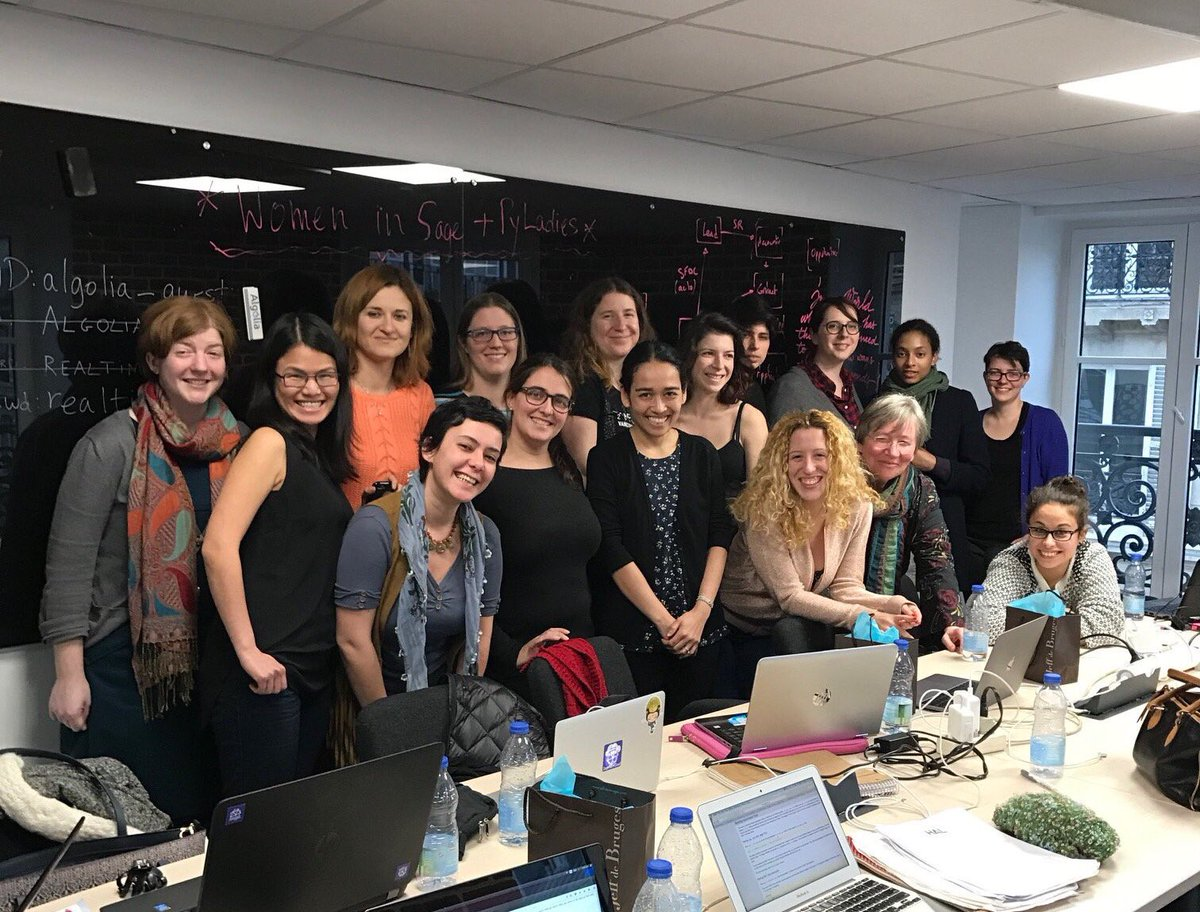
\includegraphics[scale=.2]{pyladies-WIS.jpg}
\caption*{The Women in Sage at the PyLadies coding afternoon}
\end{figure}



\end{event}
